% Options for packages loaded elsewhere
\PassOptionsToPackage{unicode}{hyperref}
\PassOptionsToPackage{hyphens}{url}
\PassOptionsToPackage{dvipsnames,svgnames,x11names}{xcolor}
%
\documentclass[
  letterpaper,
  DIV=11,
  numbers=noendperiod]{scrartcl}

\usepackage{amsmath,amssymb}
\usepackage{iftex}
\ifPDFTeX
  \usepackage[T1]{fontenc}
  \usepackage[utf8]{inputenc}
  \usepackage{textcomp} % provide euro and other symbols
\else % if luatex or xetex
  \usepackage{unicode-math}
  \defaultfontfeatures{Scale=MatchLowercase}
  \defaultfontfeatures[\rmfamily]{Ligatures=TeX,Scale=1}
\fi
\usepackage{lmodern}
\ifPDFTeX\else  
    % xetex/luatex font selection
\fi
% Use upquote if available, for straight quotes in verbatim environments
\IfFileExists{upquote.sty}{\usepackage{upquote}}{}
\IfFileExists{microtype.sty}{% use microtype if available
  \usepackage[]{microtype}
  \UseMicrotypeSet[protrusion]{basicmath} % disable protrusion for tt fonts
}{}
\makeatletter
\@ifundefined{KOMAClassName}{% if non-KOMA class
  \IfFileExists{parskip.sty}{%
    \usepackage{parskip}
  }{% else
    \setlength{\parindent}{0pt}
    \setlength{\parskip}{6pt plus 2pt minus 1pt}}
}{% if KOMA class
  \KOMAoptions{parskip=half}}
\makeatother
\usepackage{xcolor}
\setlength{\emergencystretch}{3em} % prevent overfull lines
\setcounter{secnumdepth}{-\maxdimen} % remove section numbering
% Make \paragraph and \subparagraph free-standing
\ifx\paragraph\undefined\else
  \let\oldparagraph\paragraph
  \renewcommand{\paragraph}[1]{\oldparagraph{#1}\mbox{}}
\fi
\ifx\subparagraph\undefined\else
  \let\oldsubparagraph\subparagraph
  \renewcommand{\subparagraph}[1]{\oldsubparagraph{#1}\mbox{}}
\fi

\usepackage{color}
\usepackage{fancyvrb}
\newcommand{\VerbBar}{|}
\newcommand{\VERB}{\Verb[commandchars=\\\{\}]}
\DefineVerbatimEnvironment{Highlighting}{Verbatim}{commandchars=\\\{\}}
% Add ',fontsize=\small' for more characters per line
\usepackage{framed}
\definecolor{shadecolor}{RGB}{241,243,245}
\newenvironment{Shaded}{\begin{snugshade}}{\end{snugshade}}
\newcommand{\AlertTok}[1]{\textcolor[rgb]{0.68,0.00,0.00}{#1}}
\newcommand{\AnnotationTok}[1]{\textcolor[rgb]{0.37,0.37,0.37}{#1}}
\newcommand{\AttributeTok}[1]{\textcolor[rgb]{0.40,0.45,0.13}{#1}}
\newcommand{\BaseNTok}[1]{\textcolor[rgb]{0.68,0.00,0.00}{#1}}
\newcommand{\BuiltInTok}[1]{\textcolor[rgb]{0.00,0.23,0.31}{#1}}
\newcommand{\CharTok}[1]{\textcolor[rgb]{0.13,0.47,0.30}{#1}}
\newcommand{\CommentTok}[1]{\textcolor[rgb]{0.37,0.37,0.37}{#1}}
\newcommand{\CommentVarTok}[1]{\textcolor[rgb]{0.37,0.37,0.37}{\textit{#1}}}
\newcommand{\ConstantTok}[1]{\textcolor[rgb]{0.56,0.35,0.01}{#1}}
\newcommand{\ControlFlowTok}[1]{\textcolor[rgb]{0.00,0.23,0.31}{#1}}
\newcommand{\DataTypeTok}[1]{\textcolor[rgb]{0.68,0.00,0.00}{#1}}
\newcommand{\DecValTok}[1]{\textcolor[rgb]{0.68,0.00,0.00}{#1}}
\newcommand{\DocumentationTok}[1]{\textcolor[rgb]{0.37,0.37,0.37}{\textit{#1}}}
\newcommand{\ErrorTok}[1]{\textcolor[rgb]{0.68,0.00,0.00}{#1}}
\newcommand{\ExtensionTok}[1]{\textcolor[rgb]{0.00,0.23,0.31}{#1}}
\newcommand{\FloatTok}[1]{\textcolor[rgb]{0.68,0.00,0.00}{#1}}
\newcommand{\FunctionTok}[1]{\textcolor[rgb]{0.28,0.35,0.67}{#1}}
\newcommand{\ImportTok}[1]{\textcolor[rgb]{0.00,0.46,0.62}{#1}}
\newcommand{\InformationTok}[1]{\textcolor[rgb]{0.37,0.37,0.37}{#1}}
\newcommand{\KeywordTok}[1]{\textcolor[rgb]{0.00,0.23,0.31}{#1}}
\newcommand{\NormalTok}[1]{\textcolor[rgb]{0.00,0.23,0.31}{#1}}
\newcommand{\OperatorTok}[1]{\textcolor[rgb]{0.37,0.37,0.37}{#1}}
\newcommand{\OtherTok}[1]{\textcolor[rgb]{0.00,0.23,0.31}{#1}}
\newcommand{\PreprocessorTok}[1]{\textcolor[rgb]{0.68,0.00,0.00}{#1}}
\newcommand{\RegionMarkerTok}[1]{\textcolor[rgb]{0.00,0.23,0.31}{#1}}
\newcommand{\SpecialCharTok}[1]{\textcolor[rgb]{0.37,0.37,0.37}{#1}}
\newcommand{\SpecialStringTok}[1]{\textcolor[rgb]{0.13,0.47,0.30}{#1}}
\newcommand{\StringTok}[1]{\textcolor[rgb]{0.13,0.47,0.30}{#1}}
\newcommand{\VariableTok}[1]{\textcolor[rgb]{0.07,0.07,0.07}{#1}}
\newcommand{\VerbatimStringTok}[1]{\textcolor[rgb]{0.13,0.47,0.30}{#1}}
\newcommand{\WarningTok}[1]{\textcolor[rgb]{0.37,0.37,0.37}{\textit{#1}}}

\providecommand{\tightlist}{%
  \setlength{\itemsep}{0pt}\setlength{\parskip}{0pt}}\usepackage{longtable,booktabs,array}
\usepackage{calc} % for calculating minipage widths
% Correct order of tables after \paragraph or \subparagraph
\usepackage{etoolbox}
\makeatletter
\patchcmd\longtable{\par}{\if@noskipsec\mbox{}\fi\par}{}{}
\makeatother
% Allow footnotes in longtable head/foot
\IfFileExists{footnotehyper.sty}{\usepackage{footnotehyper}}{\usepackage{footnote}}
\makesavenoteenv{longtable}
\usepackage{graphicx}
\makeatletter
\def\maxwidth{\ifdim\Gin@nat@width>\linewidth\linewidth\else\Gin@nat@width\fi}
\def\maxheight{\ifdim\Gin@nat@height>\textheight\textheight\else\Gin@nat@height\fi}
\makeatother
% Scale images if necessary, so that they will not overflow the page
% margins by default, and it is still possible to overwrite the defaults
% using explicit options in \includegraphics[width, height, ...]{}
\setkeys{Gin}{width=\maxwidth,height=\maxheight,keepaspectratio}
% Set default figure placement to htbp
\makeatletter
\def\fps@figure{htbp}
\makeatother

\KOMAoption{captions}{tableheading}
\makeatletter
\@ifpackageloaded{tcolorbox}{}{\usepackage[skins,breakable]{tcolorbox}}
\@ifpackageloaded{fontawesome5}{}{\usepackage{fontawesome5}}
\definecolor{quarto-callout-color}{HTML}{909090}
\definecolor{quarto-callout-note-color}{HTML}{0758E5}
\definecolor{quarto-callout-important-color}{HTML}{CC1914}
\definecolor{quarto-callout-warning-color}{HTML}{EB9113}
\definecolor{quarto-callout-tip-color}{HTML}{00A047}
\definecolor{quarto-callout-caution-color}{HTML}{FC5300}
\definecolor{quarto-callout-color-frame}{HTML}{acacac}
\definecolor{quarto-callout-note-color-frame}{HTML}{4582ec}
\definecolor{quarto-callout-important-color-frame}{HTML}{d9534f}
\definecolor{quarto-callout-warning-color-frame}{HTML}{f0ad4e}
\definecolor{quarto-callout-tip-color-frame}{HTML}{02b875}
\definecolor{quarto-callout-caution-color-frame}{HTML}{fd7e14}
\makeatother
\makeatletter
\makeatother
\makeatletter
\makeatother
\makeatletter
\@ifpackageloaded{caption}{}{\usepackage{caption}}
\AtBeginDocument{%
\ifdefined\contentsname
  \renewcommand*\contentsname{Table of contents}
\else
  \newcommand\contentsname{Table of contents}
\fi
\ifdefined\listfigurename
  \renewcommand*\listfigurename{List of Figures}
\else
  \newcommand\listfigurename{List of Figures}
\fi
\ifdefined\listtablename
  \renewcommand*\listtablename{List of Tables}
\else
  \newcommand\listtablename{List of Tables}
\fi
\ifdefined\figurename
  \renewcommand*\figurename{Figure}
\else
  \newcommand\figurename{Figure}
\fi
\ifdefined\tablename
  \renewcommand*\tablename{Table}
\else
  \newcommand\tablename{Table}
\fi
}
\@ifpackageloaded{float}{}{\usepackage{float}}
\floatstyle{ruled}
\@ifundefined{c@chapter}{\newfloat{codelisting}{h}{lop}}{\newfloat{codelisting}{h}{lop}[chapter]}
\floatname{codelisting}{Listing}
\newcommand*\listoflistings{\listof{codelisting}{List of Listings}}
\makeatother
\makeatletter
\@ifpackageloaded{caption}{}{\usepackage{caption}}
\@ifpackageloaded{subcaption}{}{\usepackage{subcaption}}
\makeatother
\makeatletter
\@ifpackageloaded{tcolorbox}{}{\usepackage[skins,breakable]{tcolorbox}}
\makeatother
\makeatletter
\@ifundefined{shadecolor}{\definecolor{shadecolor}{rgb}{.97, .97, .97}}
\makeatother
\makeatletter
\makeatother
\makeatletter
\makeatother
\ifLuaTeX
  \usepackage{selnolig}  % disable illegal ligatures
\fi
\IfFileExists{bookmark.sty}{\usepackage{bookmark}}{\usepackage{hyperref}}
\IfFileExists{xurl.sty}{\usepackage{xurl}}{} % add URL line breaks if available
\urlstyle{same} % disable monospaced font for URLs
\hypersetup{
  pdftitle={My Document},
  colorlinks=true,
  linkcolor={blue},
  filecolor={Maroon},
  citecolor={Blue},
  urlcolor={Blue},
  pdfcreator={LaTeX via pandoc}}

\title{My Document}
\author{}
\date{}

\begin{document}
\maketitle
\ifdefined\Shaded\renewenvironment{Shaded}{\begin{tcolorbox}[boxrule=0pt, interior hidden, enhanced, sharp corners, borderline west={3pt}{0pt}{shadecolor}, frame hidden, breakable]}{\end{tcolorbox}}\fi

\begin{tcolorbox}[enhanced jigsaw, bottomtitle=1mm, colbacktitle=quarto-callout-caution-color!10!white, toprule=.15mm, bottomrule=.15mm, toptitle=1mm, colback=white, title=\textcolor{quarto-callout-caution-color}{\faFire}\hspace{0.5em}{Expand To Learn About Collapse}, breakable, coltitle=black, opacityback=0, leftrule=.75mm, colframe=quarto-callout-caution-color-frame, arc=.35mm, rightrule=.15mm, titlerule=0mm, left=2mm, opacitybacktitle=0.6]

This is an example of a `folded' caution callout that can be expanded by
the user. You can use \texttt{collapse="true"} to collapse it by default
or \texttt{collapse="false"} to make a collapsible callout that is
expanded by default.

\end{tcolorbox}

\hypertarget{the-big-picture}{%
\section{The big picture}\label{the-big-picture}}

Now that we have completed our set up, let's dive right into programming
with \texttt{R}. In this chapter, we will go through a ``mini-project''
with very basic data, which follows a possible workflow when working
with data in \texttt{R}. We will install and load packages, load data,
perform some operations on this data, calculate some summary statistics
and plot them. In later chapters, we will go into a little more depth
for each topic. If you want to have more in depth information instead of
following the whole workflow first, you can also skip this chapter and
jump to the chapters and exercises you are interested in. But make sure
to do the final exercise, to test you R proficiency in the end.

\hypertarget{packages}{%
\subsection{Packages}\label{packages}}

\href{packages.qmd}{Packages} are extensions to the \texttt{base\ R} you
get by default. We already installed our first packages in
\href{setup.qmd\#about-this-workshop}{About this workshop}. Let's keep
doing that and install the following package as well:

\begin{Shaded}
\begin{Highlighting}[]
\FunctionTok{install.packages}\NormalTok{(}\StringTok{"tidyverse"}\NormalTok{)}
\end{Highlighting}
\end{Shaded}

The \texttt{tidyverse} is a collection of packages following a common
philosophy, and facilitate many aspects of coding in R, for example data
wrangling and plotting. We will use both functions from base R and from
the \texttt{tidyverse}. However, as i personally find them to be easier
to understand in many cases, we will use \texttt{tdiyverse} functions a
lot in the current chapter, so you can quickly get an overview of what
is possible with R.

Just by installing the packages, we can't use them. We also have to load
them into our R session:

\begin{Shaded}
\begin{Highlighting}[]
\FunctionTok{library}\NormalTok{(tidyverse)}
\end{Highlighting}
\end{Shaded}

\begin{verbatim}
-- Attaching core tidyverse packages ------------------------ tidyverse 2.0.0 --
v dplyr     1.1.2     v purrr     1.0.1
v forcats   1.0.0     v stringr   1.5.0
v ggplot2   3.4.2     v tibble    3.2.1
v lubridate 1.9.2     v tidyr     1.3.0
-- Conflicts ------------------------------------------ tidyverse_conflicts() --
x dplyr::filter() masks stats::filter()
x dplyr::lag()    masks stats::lag()
i Use the conflicted package (<http://conflicted.r-lib.org/>) to force all conflicts to become errors
\end{verbatim}

\hypertarget{load-data}{%
\subsection{Load Data}\label{load-data}}

Data is loaded into R so you can work with it. For this chapter, we are
going to use the data set \texttt{babynames}, which we can find on the
\texttt{tidytuesday} site. You can find it on
\href{https://github.com/nickhaf/r_tutorial/tree/main/raw_data}{here}.We
want to look at the most common name in every year and make a nice plot
out of it.

\begin{Shaded}
\begin{Highlighting}[]
\NormalTok{babynames }\OtherTok{\textless{}{-}} \FunctionTok{readRDS}\NormalTok{(}\StringTok{"./raw\_data/babynames.RDS"}\NormalTok{)}
\end{Highlighting}
\end{Shaded}

The above code will load the data into R and assigning it the name
\texttt{babynames} by using the \texttt{\textless{}-}. You can see the
data popping up in your \texttt{Environment} pane on the upper right.

\hypertarget{take-a-look}{%
\subsection{Take a look}\label{take-a-look}}

Now that we have our data loaded safely into R, we can get an overview
with a multitude of commands. One of the most important ones might be
\texttt{View()}, which will open the data set excel-style in a new
window:

\begin{Shaded}
\begin{Highlighting}[]
\FunctionTok{View}\NormalTok{(babynames)}
\end{Highlighting}
\end{Shaded}

Especially for bigger data sets, it might be more feasible to only look
at the structure and not the whole data set:

\begin{Shaded}
\begin{Highlighting}[]
\FunctionTok{str}\NormalTok{(babynames)}
\end{Highlighting}
\end{Shaded}

\begin{verbatim}
'data.frame':   1924665 obs. of  5 variables:
 $ year: num  NA 1880 1880 NA 1880 1880 1880 1880 1880 1880 ...
 $ sex : chr  "F" "F" "F" "F" ...
 $ name: chr  "Mary" "Anna" "Emma" "Elizabeth" ...
 $ prop: num  0.0724 0.0267 0.0205 0.0199 0.0179 ...
 $ ID  : int  1 2 3 4 5 6 7 8 9 10 ...
\end{verbatim}

On the left we can see the columns of this data.frame, named
\texttt{year}, \texttt{sex}, \texttt{names}, \texttt{n} and
\texttt{prop}. On the right we see the first values in each column, for
example \texttt{NA}, \texttt{1980}, \texttt{1980} etc \ldots{} in the
\texttt{year}-column.

\hypertarget{merging}{%
\subsection{Merging}\label{merging}}

Sadly the data is not complete. The n is missing (ok, i split it up for
illustrational purposes). So let's load it quickly:

\begin{Shaded}
\begin{Highlighting}[]
\NormalTok{babynames\_n }\OtherTok{\textless{}{-}} \FunctionTok{readRDS}\NormalTok{(}\StringTok{"./raw\_data/babynames\_n.RDS"}\NormalTok{)}
\end{Highlighting}
\end{Shaded}

And now \href{manipulation.qmd\#Merging}{merge} it:

\begin{Shaded}
\begin{Highlighting}[]
\NormalTok{babynames\_merged }\OtherTok{\textless{}{-}} \FunctionTok{merge}\NormalTok{(babynames, babynames\_n)}

\FunctionTok{head}\NormalTok{(babynames\_merged)}
\end{Highlighting}
\end{Shaded}

\begin{verbatim}
  ID year sex      name       prop    n
1  1   NA   F      Mary 0.07238359 7065
2  2 1880   F      Anna 0.02667896 2604
3  3 1880   F      Emma 0.02052149 2003
4  4   NA   F Elizabeth 0.01986579 1939
5  5 1880   F    Minnie 0.01788843 1746
6  6 1880   F  Margaret 0.01616720 1578
\end{verbatim}

Hold on! The column \texttt{years} seems to include missing values
(\texttt{NA\textquotesingle{}s}, see the cell on the top left). It is
always a good idea to deal with them before doing any analyses, so let's
do just that:

\hypertarget{missings}{%
\subsection{Missings}\label{missings}}

There are multiple ways to deal with
\href{http://localhost:5462/manipulation.html\#missing-values}{missing
values}. For reasons of simplicity, we will just remove any rows that
contain \texttt{NA\textquotesingle{}s}. We can achieve that very easily
using a function from the \texttt{tidyverse} (the package collection we
installed at the beginning of this chapter):

\begin{Shaded}
\begin{Highlighting}[]
\NormalTok{babynames\_merged }\OtherTok{\textless{}{-}} \FunctionTok{drop\_na}\NormalTok{(babynames\_merged)}
\end{Highlighting}
\end{Shaded}

\hypertarget{subsetting-data}{%
\subsection{Subsetting data}\label{subsetting-data}}

One very important part of working with data in R is the
\href{subsetting.qmd}{subsetting} of data. This means we select specific
values from a data set. Let's suppose we want to only look at the female
names in this data set:

\begin{Shaded}
\begin{Highlighting}[]
\NormalTok{babynames\_F }\OtherTok{\textless{}{-}}\NormalTok{ babynames\_merged }\SpecialCharTok{\%\textgreater{}\%}
  \FunctionTok{filter}\NormalTok{(sex }\SpecialCharTok{==} \StringTok{"F"}\NormalTok{)}
\end{Highlighting}
\end{Shaded}

\hypertarget{adding-a-new-column}{%
\subsection{Adding a new column}\label{adding-a-new-column}}

Now, we want to plot the percentages of each name, instead of the
propability, because it looks a bit more intuitive. So, let's build a
new column:

\begin{Shaded}
\begin{Highlighting}[]
\NormalTok{babynames\_F}\SpecialCharTok{$}\NormalTok{percentage }\OtherTok{\textless{}{-}}\NormalTok{ babynames\_F}\SpecialCharTok{$}\NormalTok{prop }\SpecialCharTok{*} \DecValTok{100}
\end{Highlighting}
\end{Shaded}

\hypertarget{some-additional-summary-statistics}{%
\subsection{Some additional summary
statistics}\label{some-additional-summary-statistics}}

Now, the specifics of the next part are not really relevant. However,
they can show you how easy it can be to deal with data in R: First,
let's group our data according to year:

\begin{Shaded}
\begin{Highlighting}[]
\NormalTok{babynames\_F\_grouped }\OtherTok{\textless{}{-}}\NormalTok{ babynames\_F }\SpecialCharTok{\%\textgreater{}\%}
  \FunctionTok{group\_by}\NormalTok{(year)}
\end{Highlighting}
\end{Shaded}

Any operations we now perform are performed for every group. In our
case, we want to find the name with the maximum \texttt{prop} in each
group:

\begin{Shaded}
\begin{Highlighting}[]
\NormalTok{babynames\_F\_max }\OtherTok{\textless{}{-}}\NormalTok{ babynames\_F\_grouped }\SpecialCharTok{\%\textgreater{}\%}
  \FunctionTok{slice}\NormalTok{(}\FunctionTok{which.max}\NormalTok{(percentage))}

\FunctionTok{head}\NormalTok{(babynames\_F\_max)}
\end{Highlighting}
\end{Shaded}

\begin{verbatim}
# A tibble: 6 x 7
# Groups:   year [6]
     ID  year sex   name    prop     n percentage
  <int> <dbl> <chr> <chr>  <dbl> <dbl>      <dbl>
1     2  1880 F     Anna  0.0267  2604       2.67
2  2001  1881 F     Mary  0.0700  6919       7.00
3  3936  1882 F     Mary  0.0704  8148       7.04
4  6063  1883 F     Mary  0.0667  8012       6.67
5  8147  1884 F     Mary  0.0670  9217       6.70
6 10444  1885 F     Mary  0.0643  9128       6.43
\end{verbatim}

Great! We now have a data frame containing one row for every year. In
it, we find the name most common in that year. As already mentioned, the
specifics of these functions are not really relevant for this workshop.

\hypertarget{plot-the-data}{%
\subsection{Plot the data}\label{plot-the-data}}

This section is more additional and not really necessary for the other
workshops. However, i think it is a great way to show you the beauty of
plotting in R, so here it goes (make sure you worked on the other
concepts first).

We will use the package \texttt{ggplot2} (which is also part of the
\texttt{tidyverse}) for plotting our data. It should be mentioned that
\texttt{Base\ R} also has some powerful plotting functions, however,
\texttt{ggplot2} makes it very easy to build complex and beautiful
plots.

A ggplot is constructed from multiple layers, that can be laid over each
other using the \texttt{+} operator.

We start with the function \texttt{ggplot()}, where we define our data
and the x and y aestetics.

\begin{Shaded}
\begin{Highlighting}[]
\NormalTok{p }\OtherTok{\textless{}{-}} \FunctionTok{ggplot}\NormalTok{(}
  \AttributeTok{data =}\NormalTok{ babynames\_F\_max,}
  \FunctionTok{aes}\NormalTok{(}
    \AttributeTok{x =}\NormalTok{ year,}
    \AttributeTok{y =}\NormalTok{ percentage)}
\NormalTok{  )}
\end{Highlighting}
\end{Shaded}

We can also define different colours for different groups. For example,
if we want the bars to get filled with a colour corresponding to the
name they are representing, we can do that:

\begin{Shaded}
\begin{Highlighting}[]
\NormalTok{p }\OtherTok{\textless{}{-}} \FunctionTok{ggplot}\NormalTok{(}
  \AttributeTok{data =}\NormalTok{ babynames\_F\_max,}
  \FunctionTok{aes}\NormalTok{(}
    \AttributeTok{x =}\NormalTok{ year,}
    \AttributeTok{y =}\NormalTok{ percentage,}
    \AttributeTok{fill =}\NormalTok{ name}
\NormalTok{  )}
\NormalTok{)}
\end{Highlighting}
\end{Shaded}

Now that we have defined our aesthetics, we can add a
\texttt{geom}-layer. This will make use of the data we have defined in
\texttt{ggplot()} and plot some bars for us:

\begin{Shaded}
\begin{Highlighting}[]
\NormalTok{p }\OtherTok{\textless{}{-}}\NormalTok{ p }\SpecialCharTok{+}
  \FunctionTok{geom\_col}\NormalTok{()}
\NormalTok{p}
\end{Highlighting}
\end{Shaded}

\begin{figure}[H]

{\centering 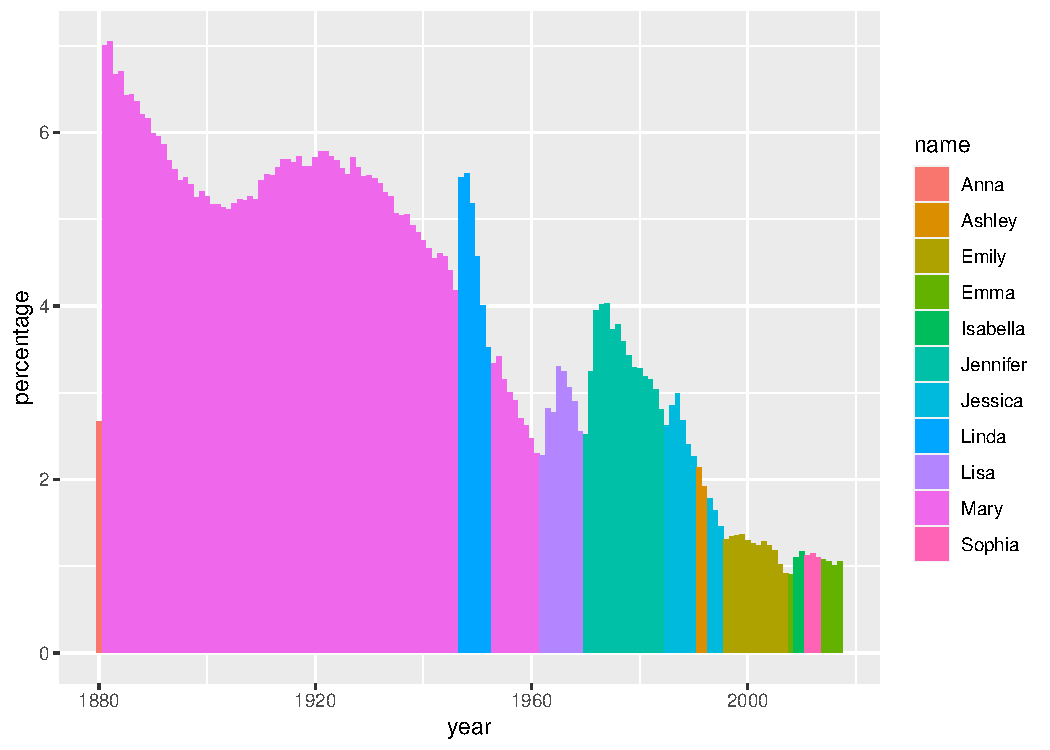
\includegraphics{the_big_picture_files/figure-pdf/unnamed-chunk-13-1.pdf}

}

\end{figure}

Let's give the axes some more informative names and a title to the plot:

\begin{Shaded}
\begin{Highlighting}[]
\NormalTok{p }\OtherTok{\textless{}{-}}\NormalTok{ p }\SpecialCharTok{+}
  \FunctionTok{ggtitle}\NormalTok{(}\StringTok{"Most common female name in the United States of America by year"}\NormalTok{) }\SpecialCharTok{+}
  \FunctionTok{xlab}\NormalTok{(}\StringTok{"Birthyear"}\NormalTok{) }\SpecialCharTok{+}
  \FunctionTok{ylab}\NormalTok{(}\StringTok{"Percentage of children given that name relative to total births"}\NormalTok{)}
\NormalTok{p}
\end{Highlighting}
\end{Shaded}

\begin{figure}[H]

{\centering 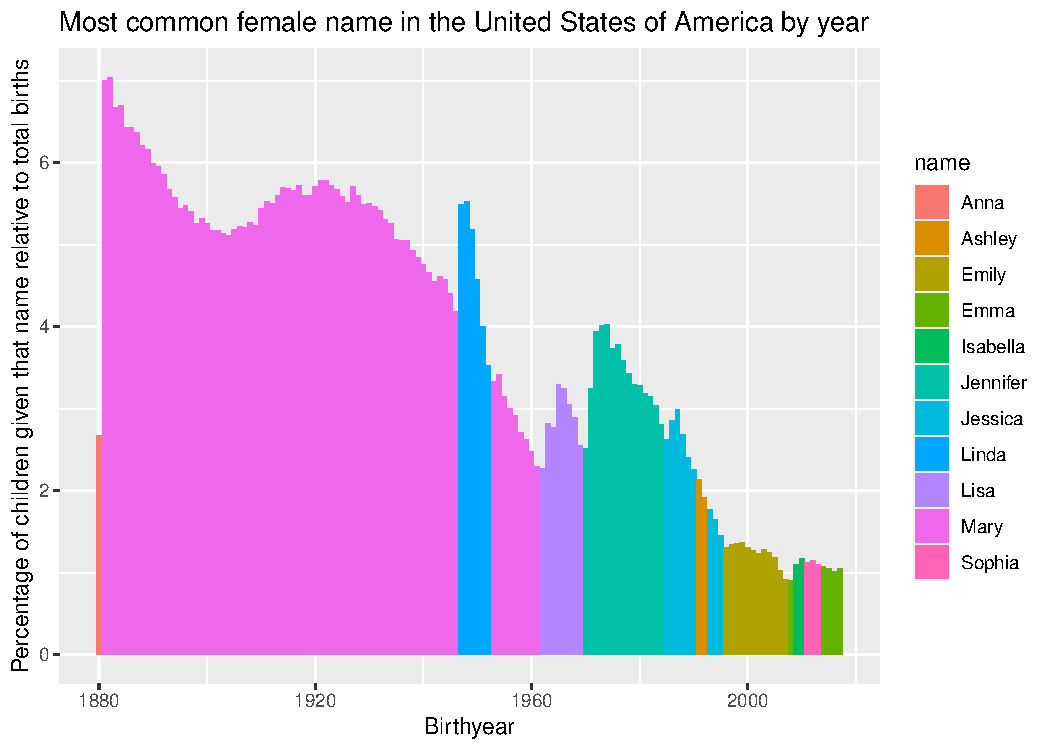
\includegraphics{the_big_picture_files/figure-pdf/unnamed-chunk-14-1.pdf}

}

\end{figure}

Finally, to style the plot a bit, let's add a predefined theme and a
color palette:

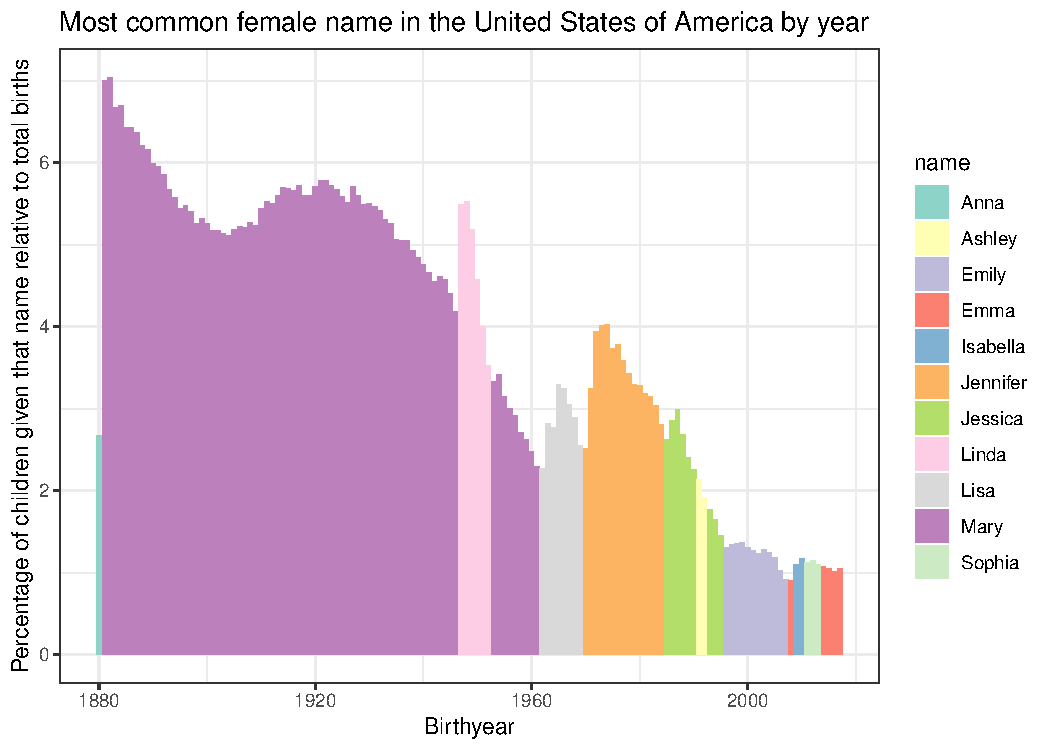
\includegraphics{the_big_picture_files/figure-pdf/plot-smaller-diamonds-1.pdf}

\hypertarget{conclusion}{%
\subsection{Conclusion}\label{conclusion}}

In this tutorial we learned, that R is a flexible tool for editing and
plotting data. Of course, we barely scratched the surface. Therefore, we
want to dive a bit deeper into each step. Either follow the course, or
navigate to the chapters you are most interested in.

Foto von Mick Haupt auf Unsplash

\hypertarget{final-exercise}{%
\subsection{Final Exercise}\label{final-exercise}}

\begin{Shaded}
\begin{Highlighting}[]
\CommentTok{\# Für die Übung.}
\CommentTok{\# install.packages("tidytuesdayR")}
\FunctionTok{library}\NormalTok{(tidytuesdayR)}
\NormalTok{tuesdata }\OtherTok{\textless{}{-}}\NormalTok{ tidytuesdayR}\SpecialCharTok{::}\FunctionTok{tt\_load}\NormalTok{(}\StringTok{"2022{-}08{-}16"}\NormalTok{)}
\end{Highlighting}
\end{Shaded}




\end{document}
